\section{Actividad nro 2 - SEGUNDO LATEX}

\vspace*{0.1in}
\begin{large}
 El control de versiones es un sistema que registra los cambios realizados sobre un archivo o conjunto de archivos a lo largo del tiempo, de modo que puedas recuperar versiones específicas más adelante. Te permite revertir archivos a un estado anterior, revertir el proyecto entero a un estado anterior, comparar cambios a lo largo del tiempo.\\
\end{large}


\begin{itemize}
	\item PERÚ
	\\Parte del mundial 
	\begin{center}
	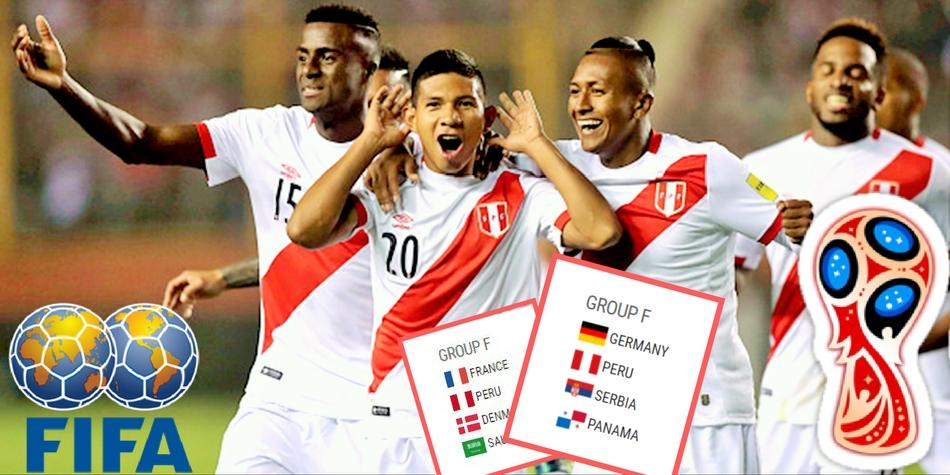
\includegraphics[width=15cm]{./Imagenes/act2_1} 
	\end{center}

\end{itemize}